\documentclass[12pt]{article} % use larger type; default would be 10pt

\usepackage{tikz}
\usepackage{pgfplots}
\usetikzlibrary{calc}
\usetikzlibrary{arrows.meta}
\usetikzlibrary{patterns}
        \newcommand\degree[0]{^{\circ}}
\usetikzlibrary{shapes.misc}

\title{Play with TikZ}
\author{Just Us}
%\date{} % Activate to display a given date or no date (if empty),
         % otherwise the current date is printed 

\begin{document}
\maketitle

\section{Chap 4 Trigonometric Functions}

\subsection{4.3 Periodic functions}


exam4-3-1a two scaled sine graphs

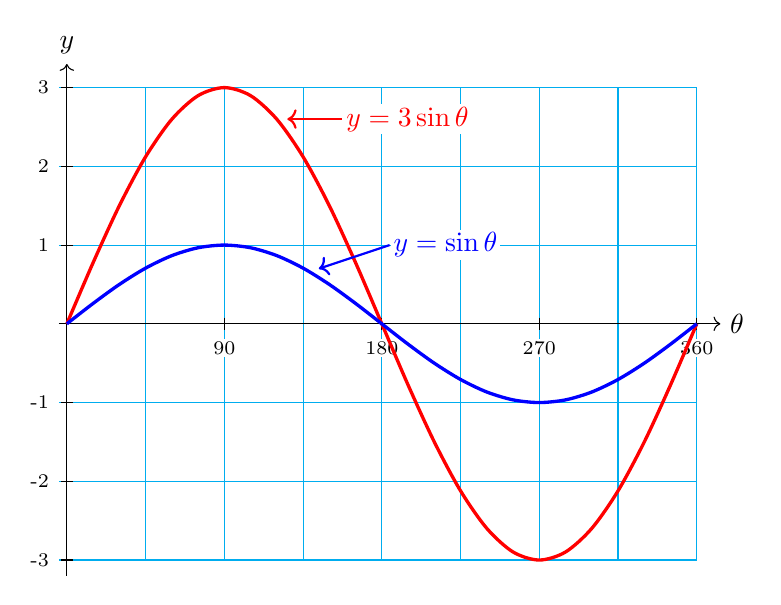
\begin{tikzpicture} 
\draw[cyan]
(-0.1,-3) grid (8,3);

\draw[->] (-0.1,0) -- (8.3,0) node[right] {$\theta$};
\draw[->] (0,-3.2) -- (0,3.3) node[above] {$y$};

\foreach \x [evaluate=\x as \xi using int( 45* \x )] in {2, 4, 6, 8}
\draw[black] ($ \x *(1,0) +(0,.08) $) --++(0,-.16) node[anchor=north, xshift=0,yshift=-3, fill=white, inner sep=1pt] {\scriptsize$ \xi $};

\foreach \y  [evaluate=\y as \yi using int(  \y )] in {-3, -2, -1,1, 2, 3}
\draw[black] (.08,\y ) --++(-.16,0) node[anchor=east, xshift=-3, fill=white, inner sep=1pt] {\scriptsize\yi};

\draw[domain=-0:8,smooth,variable=\x,red,very thick] plot ({\x},{ 3*sin(deg(\x*pi/4))});

\draw[red, thick, <-] (2.8, 2.6) -- +(0.7,0) node[right, fill=white, inner sep=1pt] {$y=3\sin \theta$};
\draw[domain=-0:8,smooth,variable=\x,blue,very thick] plot ({\x},{ sin(deg(\x*pi/4))});
\draw[blue, thick, <-] (3.2, 0.7) -- +(0.9,0.3) node[right, fill=white, inner sep=1pt] {$y=\sin \theta$};

\end{tikzpicture}
\newline

exam4-3-1b sine and 3+ sine

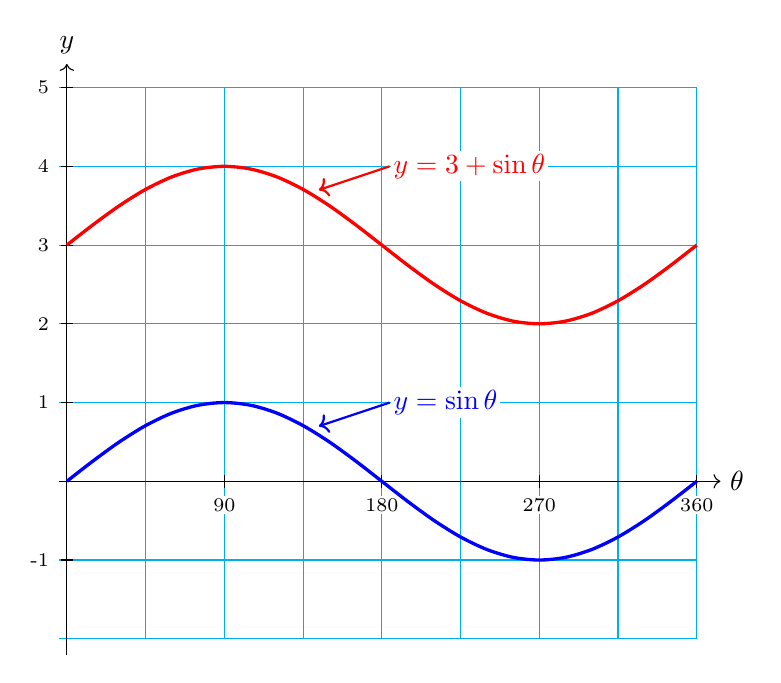
\begin{tikzpicture} 
\draw[cyan]
(-0.1,-2) grid (8,5);

\draw[->] (-0.1,0) -- (8.3,0) node[right] {$\theta$};
\draw[->] (0,-2.2) -- (0,5.3) node[above] {$y$};

\foreach \x [evaluate=\x as \xi using int( 45* \x )] in {2, 4, 6, 8}
\draw[black] ($ \x *(1,0) +(0,.08) $) --++(0,-.16) node[anchor=north, xshift=0,yshift=-3, fill=white, inner sep=1pt] {\scriptsize$ \xi $};

\foreach \y  [evaluate=\y as \yi using int(  \y )] in { -1,1, 2, 3, 4, 5}
\draw[black] (.08,\y ) --++(-.16,0) node[anchor=east, xshift=-3, fill=white, inner sep=1pt] {\scriptsize\yi};

\draw[domain=-0:8,smooth,variable=\x,red,very thick] plot ({\x},{ 3+sin(deg(\x*pi/4))});
\draw[red, thick, <-] (3.2, 3.7) -- +(0.9,0.3) node[right, fill=white, inner sep=1pt] {$y=3+\sin \theta$};

\draw[domain=-0:8,smooth,variable=\x,blue,very thick] plot ({\x},{ sin(deg(\x*pi/4))});
\draw[blue, thick, <-] (3.2, 0.7) -- +(0.9,0.3) node[right, fill=white, inner sep=1pt] {$y=\sin \theta$};

\end{tikzpicture}
\newline

exam4-3-1c sine and  sine 3 theta

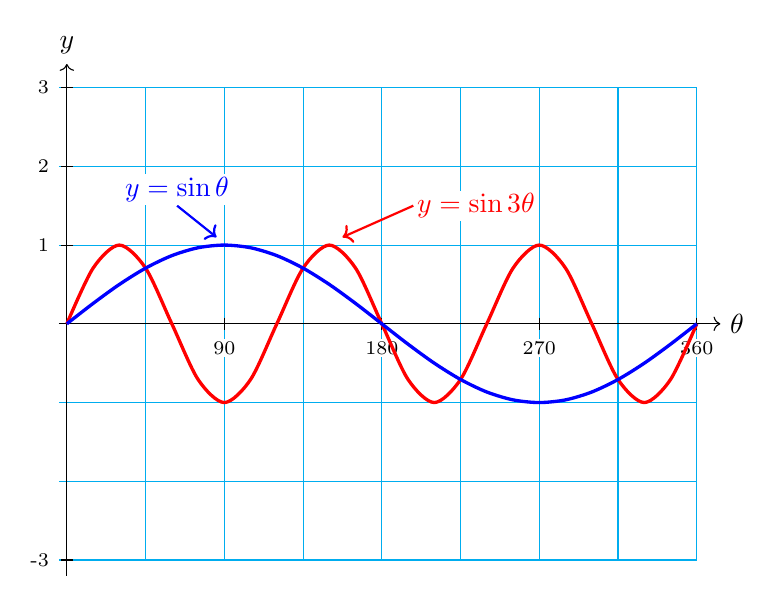
\begin{tikzpicture} 
\draw[cyan]
(-0.1,-3) grid (8,3);

\draw[->] (-0.1,0) -- (8.3,0) node[right] {$\theta$};
\draw[->] (0,-3.2) -- (0,3.3) node[above] {$y$};

\foreach \x [evaluate=\x as \xi using int( 45* \x )] in {2, 4, 6, 8}
\draw[black] ($ \x *(1,0) +(0,.08) $) --++(0,-.16) node[anchor=north, xshift=0,yshift=-3, fill=white, inner sep=1pt] {\scriptsize$ \xi $};

\foreach \y  [evaluate=\y as \yi using int(  \y )] in {-3, -2 -1,1, 2, 3 }
\draw[black] (.08,\y ) --++(-.16,0) node[anchor=east, xshift=-3, fill=white, inner sep=1pt] {\scriptsize\yi};

\draw[domain=-0:8,smooth,variable=\x,red,very thick] plot ({\x},{ sin(deg(\x*3*pi/4))});
\draw[red, thick, <-] (3.5, 1.1) -- +(0.9,0.4) node[right, fill=white, inner sep=1pt] {$y=\sin 3 \theta$};

\draw[domain=-0:8,smooth,variable=\x,blue,very thick] plot ({\x},{ sin(deg(\x*pi/4))});
\draw[blue, thick, <-] (1.9, 1.1) -- +(-0.5,0.4) node[above, fill=white, inner sep=1pt] {$y=\sin \theta$};

\end{tikzpicture}
\newline

exam4-3-2 $-3 + 4\sin 3\theta$

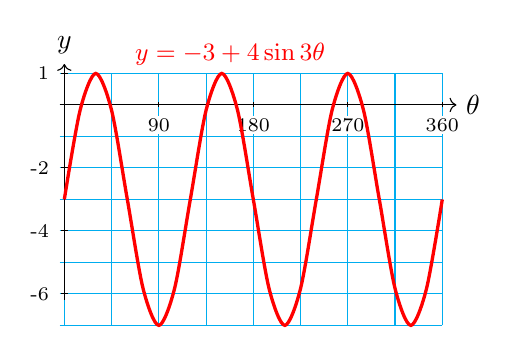
\begin{tikzpicture} [xscale=.6, yscale=.4]
\draw[cyan]
(-0.1,-7) grid (8,1);

\draw[->] (-0.1,0) -- (8.3,0) node[right] {$\theta$};
\draw[->] (0,-6.2) -- (0,1.3) node[above] {$y$};

\foreach \x [evaluate=\x as \xi using int( 45* \x )] in {2, 4, 6, 8}
\draw[black] ($ \x *(1,0) +(0,.08) $) --++(0,-.16) node[anchor=north, xshift=0,yshift=-3, fill=white, inner sep=1pt] {\scriptsize$ \xi $};

\foreach \y  [evaluate=\y as \yi using int(  \y )] in { -6, -4, -2,1}
\draw[black] (.08,\y ) --++(-.16,0) node[anchor=east, xshift=-3, fill=white, inner sep=1pt] {\scriptsize\yi};

\draw[domain=-0:8,smooth,variable=\x,red,very thick] plot ({\x},{ -3+4*sin(deg(\x*3*pi/4))});

\node [text width= 3cm, text=red] at (4, 1.6){\small $y=-3+4\sin 3 \theta$};


\end{tikzpicture}
\newline

exer4-3-1ansa cosine +2

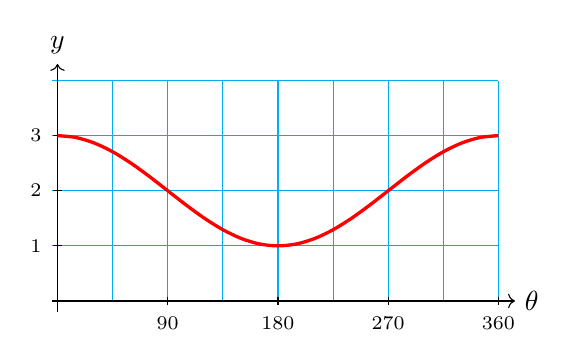
\begin{tikzpicture} [scale=0.7]
\draw[cyan]
(-0.1,0) grid (8,4);

\draw[->] (-0.1,0) -- (8.3,0) node[right] {$\theta$};
\draw[->] (0,-.2) -- (0,4.3) node[above] {$y$};

\foreach \x [evaluate=\x as \xi using int( 45* \x )] in {2, 4, 6, 8}
\draw[black] ($ \x *(1,0) +(0,.08) $) --++(0,-.16) node[anchor=north, xshift=0,yshift=-3, fill=white, inner sep=1pt] {\scriptsize$ \xi $};

\foreach \y  [evaluate=\y as \yi using int(  \y )] in {1, 2, 3 }
\draw[black] (.08,\y ) --++(-.16,0) node[anchor=east, xshift=-3, fill=white, inner sep=1pt] {\scriptsize\yi};

\draw[domain=-0:8,smooth,variable=\x,red,very thick] plot ({\x},{ 2+cos(deg(\x*pi/4))});

\end{tikzpicture}
\newline

exer4-3-1ansb cosine 2 theta

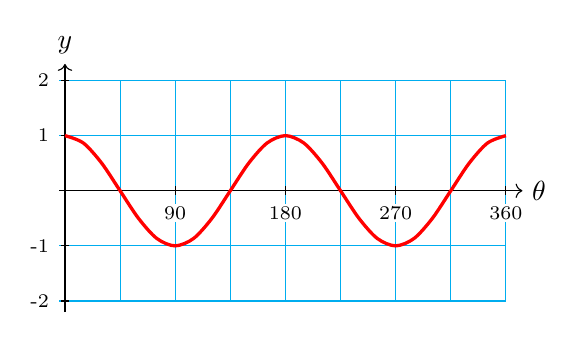
\begin{tikzpicture} [scale=0.7]
\draw[cyan]
(-0.1,-2) grid (8,2);

\draw[->] (-0.1,0) -- (8.3,0) node[right] {$\theta$};
\draw[->] (0,-2.2) -- (0,2.3) node[above] {$y$};

\foreach \x [evaluate=\x as \xi using int( 45* \x )] in {2, 4, 6, 8}
\draw[black] ($ \x *(1,0) +(0,.08) $) --++(0,-.16) node[anchor=north, xshift=0,yshift=-3, fill=white, inner sep=1pt] {\scriptsize$ \xi $};

\foreach \y  [evaluate=\y as \yi using int(  \y )] in { -2, -1, 1, 2 }
\draw[black] (.08,\y ) --++(-.16,0) node[anchor=east, xshift=-3, fill=white, inner sep=1pt] {\scriptsize\yi};

\draw[domain=-0:8,smooth,variable=\x,red,very thick] plot ({\x},{ cos(deg(\x*2*pi/4))});

\end{tikzpicture}
\newline

exer4-3-1ansc 2 cosine theta

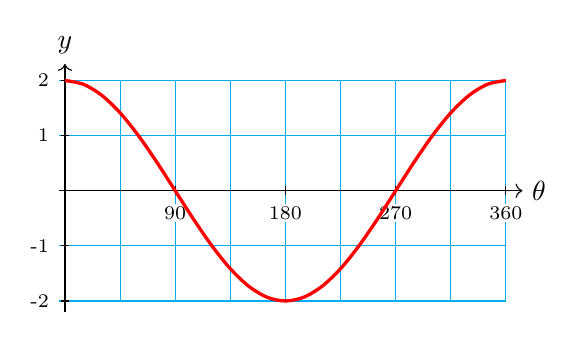
\begin{tikzpicture} [scale=0.7]
\draw[cyan]
(-0.1,-2) grid (8,2);

\draw[->] (-0.1,0) -- (8.3,0) node[right] {$\theta$};
\draw[->] (0,-2.2) -- (0,2.3) node[above] {$y$};

\foreach \x [evaluate=\x as \xi using int( 45* \x )] in {2, 4, 6, 8}
\draw[black] ($ \x *(1,0) +(0,.08) $) --++(0,-.16) node[anchor=north, xshift=0,yshift=-3, fill=white, inner sep=1pt] {\scriptsize$ \xi $};

\foreach \y  [evaluate=\y as \yi using int(  \y )] in { -2, -1, 1, 2 }
\draw[black] (.08,\y ) --++(-.16,0) node[anchor=east, xshift=-3, fill=white, inner sep=1pt] {\scriptsize\yi};

\draw[domain=-0:8,smooth,variable=\x,red,very thick] plot ({\x},{ 2*cos(deg(\x*pi/4))});

\end{tikzpicture}
\newline

exer4-3-2ans $y = 1 - 3\sin 2\theta$

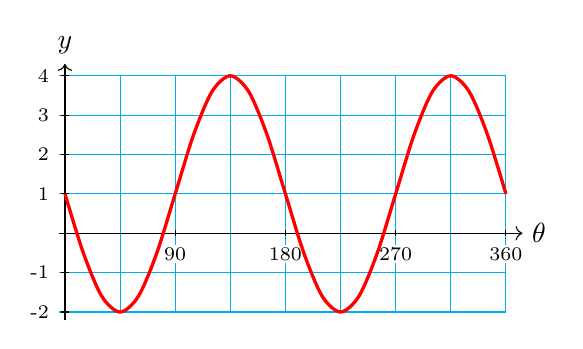
\begin{tikzpicture} [xscale=0.7, yscale=.5]
\draw[cyan] (-0.1,-2) grid (8,4);

\draw[->] (-0.1,0) -- (8.3,0) node[right] {$\theta$};
\draw[->] (0,-2.2) -- (0,4.3) node[above] {$y$};

\foreach \x [evaluate=\x as \xi using int( 45* \x )] in {2, 4, 6, 8}
\draw[black] ($ \x *(1,0) +(0,.08) $) --++(0,-.16) node[anchor=north, xshift=0,yshift=-3, fill=white, inner sep=1pt] {\scriptsize$ \xi $};

\foreach \y  [evaluate=\y as \yi using int(  \y )] in { -2, -1, 1, 2,3,4 }
\draw[black] (.08,\y ) --++(-.16,0) node[anchor=east, xshift=-3, fill=white, inner sep=1pt] {\scriptsize\yi};

\draw[domain=-0:8,smooth,variable=\x,red,very thick] plot ({\x},{ 1-3*sin(deg(\x*2*pi/4))});

\end{tikzpicture}
\newline

exam4-3-3 graphs

\begin{tikzpicture} 
\coordinate (O) at (0,0);

\draw[->] (O)++(-1.5,0) -- +(3.2,0) node[right] {$t$};
\draw[->] (O)++(0,-0.1) -- +(0,3.3) node[above] {$h$};

\draw[red, very thick] (O)++(0,2) circle (.7 cm);
\node[text width=.2 cm] at (0,-.6) {a.};

% second graph
\coordinate (O) at (4.2,0);

\draw[->] (O)++(-0.2,0) -- +(3.2,0) node[right] {$t$};
\draw[->] (O)++(0,-0.1) -- +(0,3.3) node[above] {$h$};

\draw[red, very thick] (O)++(0,2.7) --++(.6,-1.4)--++(.6,1.4)--++(.6,-1.4)--++(.6,1.4)--++(.12,-0.28);

\node[text width=.2 cm] at ($(O)+(1.5,-.6)$) {b.};

% third graph
\coordinate (O) at (9.4,0);

\draw[->] (O)++(-0.2,0) -- +(3.2,0) node[right] {$t$};
\draw[->] (O)++(0,-0.1) -- +(0,3.3) node[above] {$h$};

\draw[domain=9.4:12.2,smooth,variable=\x,red,very thick] plot ({\x},{2+ 0.7*cos(deg((\x- 9.4)*4.8))});
\node[text width=.2 cm] at ($(O)+(1.5,-.6)$) {c.};

\end{tikzpicture}
\newline

exam4-3-3soln clock
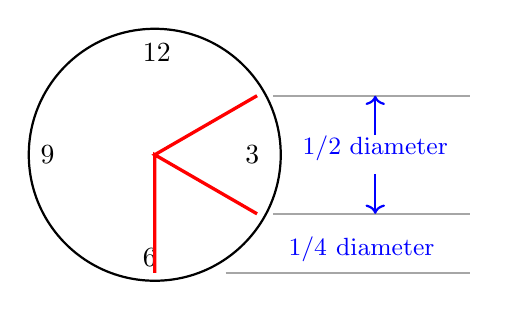
\begin{tikzpicture}
\coordinate (O) at (0,0);
\draw[black, thick] (O) circle (1.6 cm);

\foreach \theta [evaluate=\theta as \h using int(3*\theta )]  in {1, 2, 3, 4}  {
  \node[text width = .3cm] at (-90*\theta+90:1.3){\h}; }

\coordinate (h2) at (30:1.5);
\coordinate (h4) at (-30:1.5);
\coordinate (h6) at (-90:1.5);

\draw[red, very thick] (h2)--(O)--(h4)--(O)--(h6);

\coordinate (P) at ($ (1.5,0)+ 1.5*sin(30)*(0,1) $);
\coordinate (Q) at ($ (1.5,0)+ 1.5*sin(30)*(0,-1) $);
\coordinate (R) at (0.9,-1.5);

\draw[gray!70!white, thick] (P) -- +(2.5,0);
\draw[gray!70!white, thick] (Q) -- +(2.5,0);
\draw[blue, thick, <-] (P)++(1.3,0) --+(0,-.5) node[below, fill=white, inner sep=0] {\small 1/2 diameter};
\draw[blue, thick, <-] (Q)++(1.3,0) --+(0,.5);
\draw[gray!70!white, thick] (R) -- +(3.1,0);
\node[text width = 2.4cm, text=blue] at (2.9,-1.2){\small 1/4 diameter};

\end{tikzpicture}
\newline

exer4-3-3a sinusoidal graph

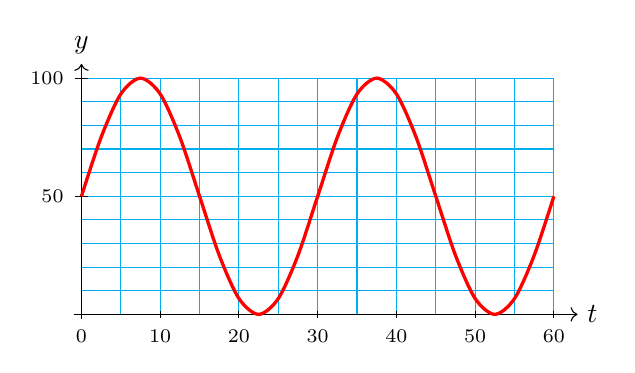
\begin{tikzpicture} [yscale=.6]
\draw[cyan, xstep=.5, ystep=.5] (0,0) grid (6,5);

\draw[->] (-0.1,0) -- (6.3,0) node[right] {$t$};
\draw[->] (0,-.1) -- (0,5.3) node[above] {$y$};

\foreach \x [evaluate=\x as \xi using int( 10* \x )] in {0, 1, 2, ..., 6}
\draw[black] ($ \x *(1,0) +(0,.08) $) --++(0,-.16) node[anchor=north, xshift=0,yshift=-3, fill=white, inner sep=1pt] {\scriptsize$ \xi $};

\foreach \y  [evaluate=\y as \yi using int( 20* \y )] in {2.5,5}
\draw[black] (.08,\y ) --++(-.16,0) node[anchor=east, xshift=-3, fill=white, inner sep=1pt] {\scriptsize\yi};

\draw[domain=-0:6,smooth,variable=\x,red,very thick] plot ({\x},{ 2.5+2.5*sin(deg(\x*2*pi/3))});

\end{tikzpicture}
\newline

exer4-3-3b sinusoidal graph

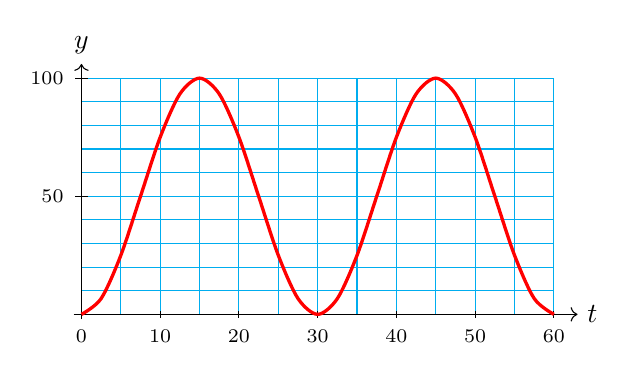
\begin{tikzpicture} [yscale=.6]
\draw[cyan, xstep=.5, ystep=.5] (0,0) grid (6,5);

\draw[->] (-0.1,0) -- (6.3,0) node[right] {$t$};
\draw[->] (0,-.1) -- (0,5.3) node[above] {$y$};

\foreach \x [evaluate=\x as \xi using int( 10* \x )] in {0, 1, 2, ..., 6}
\draw[black] ($ \x *(1,0) +(0,.08) $) --++(0,-.16) node[anchor=north, xshift=0,yshift=-3, fill=white, inner sep=1pt] {\scriptsize$ \xi $};

\foreach \y  [evaluate=\y as \yi using int( 20* \y )] in {2.5,5}
\draw[black] (.08,\y ) --++(-.16,0) node[anchor=east, xshift=-3, fill=white, inner sep=1pt] {\scriptsize\yi};

\draw[domain=-0:6,smooth,variable=\x,red,very thick] plot ({\x},{ 2.5-2.5*cos(deg(\x*2*pi/3))});

\end{tikzpicture}
\newline

exer4-3-3c sinusoidal graph

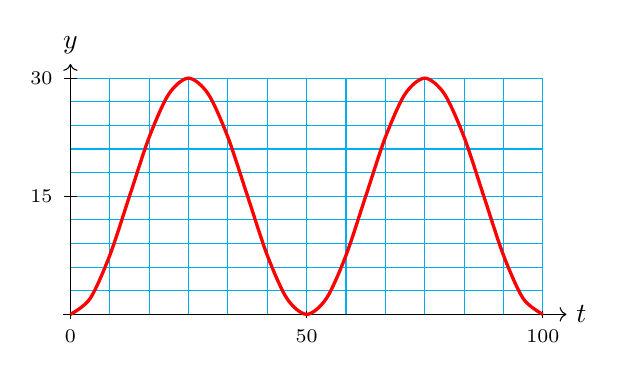
\begin{tikzpicture} [yscale=.6]
\draw[cyan, xstep=.5, ystep=.5] (0,0) grid (6,5);

\draw[->] (-0.1,0) -- (6.3,0) node[right] {$t$};
\draw[->] (0,-.1) -- (0,5.3) node[above] {$y$};

\foreach \x [evaluate=\x as \xi using int( 50* \x /3)] in {0, 3, 6}
\draw[black] ($ \x *(1,0) +(0,.08) $) --++(0,-.16) node[anchor=north, xshift=0,yshift=-3, fill=white, inner sep=1pt] {\scriptsize$ \xi $};

\foreach \y  [evaluate=\y as \yi using int( 6* \y )] in {2.5,5}
\draw[black] (.08,\y ) --++(-.16,0) node[anchor=east, xshift=-3, fill=white, inner sep=1pt] {\scriptsize\yi};

\draw[domain=-0:6,smooth,variable=\x,red,very thick] plot ({\x},{ 2.5-2.5*cos(deg(\x*2*pi/3))});

\end{tikzpicture}
\newline


exam4-3-4 sinusoidal graph

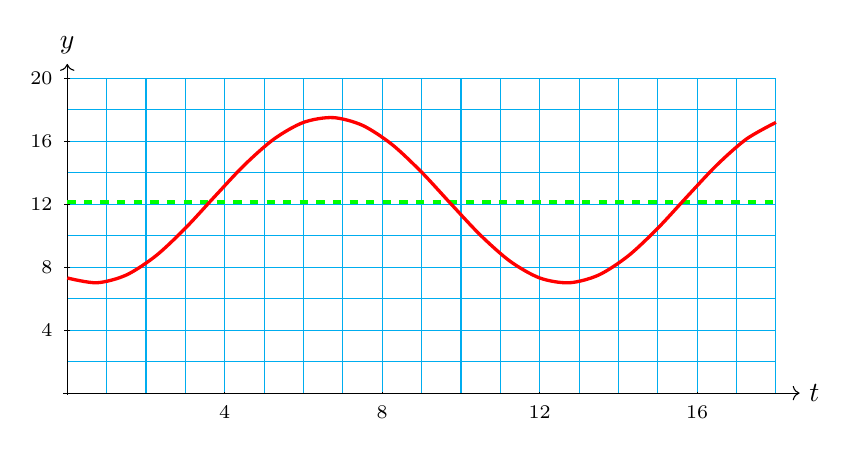
\begin{tikzpicture} [xscale=.5, yscale=.2] 
\draw[cyan, xstep=1, ystep=2] (0,0) grid (18,20);

\draw[->] (-0.1,0) -- (18.6,0) node[right] {$t$};
\draw[->] (0,-.1) -- (0,20.9) node[above] {$y$};
\draw[green, ultra thick, dashed] (0,12.12)--+(18,0);

\foreach \x [evaluate=\x as \xi using int( 1* \x /1)] in {4, 8, ..., 16}
\draw[black] ($ \x *(1,0) +(0,.08) $) --++(0,-.16) node[anchor=north, xshift=0,yshift=-3, fill=white, inner sep=1pt] {\scriptsize$ \xi $};

\foreach \y  [evaluate=\y as \yi using int( 1* \y )] in {4, 8,..., 20}
\draw[black] (.08,\y ) --++(-.16,0) node[anchor=east, xshift=-3, fill=white, inner sep=1pt] {\scriptsize\yi};

\draw[domain=-0:18,smooth,variable=\x,red,very thick] plot ({\x},{ 12.25-5.25*cos(deg((\x-.66)*pi/6))});

\end{tikzpicture}
\newline

\section{Algebra refresher graphs}
ar4-3-1ans $f(x) = \frac{1}{x - 2}$
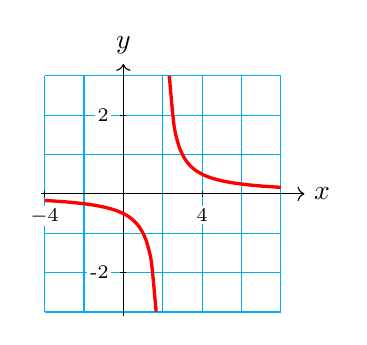
\begin{tikzpicture} [scale=.5]
\draw[cyan] (-2,-3) grid (4,3);

\draw[->] (-2.1,0) -- (4.6,0) node[right] {$x$};
\draw[->] (0,-3.1) -- (0,3.3) node[above] {$y$};

\foreach \x [evaluate=\x as \xi using int( 2* \x )] in {-2,2} \draw[black] ($ \x *(1,0) +(0,.08) $) --++(0,-.16) node[anchor=north, xshift=0,yshift=-3, fill=white, inner sep=1pt] {\scriptsize$ \xi $};

\foreach \y [evaluate=\y as \yi using int( 1* \y )]   in {-2, 2} \draw[black] (.08,\y ) --++(-.16,0) node[anchor=east, xshift=-3, fill=white, inner sep=1pt] {\scriptsize\yi};

\draw[domain={-2:5/6},smooth,variable=\x,red,very thick] plot ({\x},{1/(2*\x-2)});

\draw[domain={7/6:4},smooth,variable=\x,red,very thick] plot ({\x},{1/(2*\x-2)});
\end{tikzpicture}
\newline


ar4-3-2ans $f(x) = \frac{1}{x +3}$
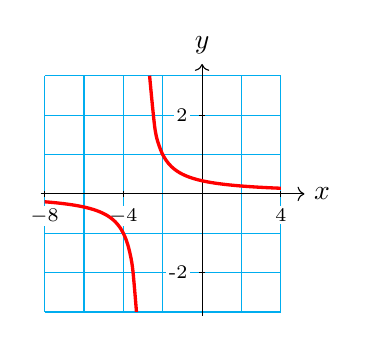
\begin{tikzpicture} [scale=.5]
\draw[cyan] (-4,-3) grid (2,3);

\draw[->] (-4.1,0) -- (2.6,0) node[right] {$x$};
\draw[->] (0,-3.1) -- (0,3.3) node[above] {$y$};

\foreach \x [evaluate=\x as \xi using int( 2* \x )] in {-4,-2,2} \draw[black] ($ \x *(1,0) +(0,.08) $) --++(0,-.16) node[anchor=north, xshift=0,yshift=-3, fill=white, inner sep=1pt] {\scriptsize$ \xi $};

\foreach \y [evaluate=\y as \yi using int( 1* \y )]   in {-2, 2} \draw[black] (.08,\y ) --++(-.16,0) node[anchor=east, xshift=-3, fill=white, inner sep=1pt] {\scriptsize\yi};

\draw[domain={-4:-5/3},smooth,variable=\x,red,very thick] plot ({\x},{1/(2*\x +3)});

\draw[domain={-8/6:2},smooth,variable=\x,red,very thick] plot ({\x},{1/(2*\x +3)});
\end{tikzpicture}
\newline


ar4-3-3ans $f(x) = \frac{1}{x^2 -1}$
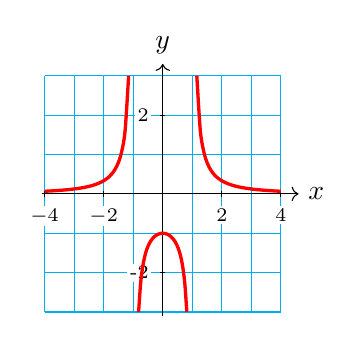
\begin{tikzpicture} [xscale=.375, yscale=.5]
\draw[cyan] (-4,-3) grid (4,3);

\draw[->] (-4.1,0) -- (4.6,0) node[right] {$x$};
\draw[->] (0,-3.1) -- (0,3.3) node[above] {$y$};

\foreach \x [evaluate=\x as \xi using int(  \x )] in {-4,-2,2,4} \draw[black] ($ \x *(1,0) +(0,.08) $) --++(0,-.16) node[anchor=north, xshift=0,yshift=-3, fill=white, inner sep=1pt] {\scriptsize$ \xi $};

\foreach \y [evaluate=\y as \yi using int( 1* \y )]   in {-2, 2} \draw[black] (.08,\y ) --++(-.16,0) node[anchor=east, xshift=-3, fill=white, inner sep=1pt] {\scriptsize\yi};

\draw[domain={-4:-2/sqrt(3)},smooth,variable=\x,red,very thick] plot ({\x},{1/( (\x)^2 -1)});

\draw[domain={-sqrt(2/3):sqrt(2/3)},smooth,variable=\x,red,very thick] plot ({\x},{1/( (\x)^2 -1)});

\draw[domain={2/sqrt(3):4},smooth,variable=\x,red,very thick] plot ({\x},{1/( (\x)^2 -1)});
\end{tikzpicture}
\newline


ar4-3-4ans $f(x) = \frac{-1}{(x+1)^2 }$
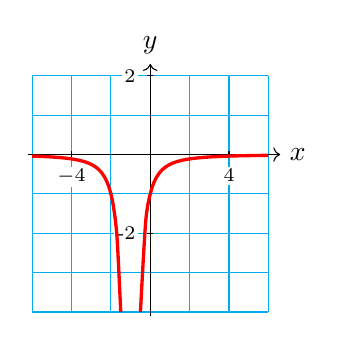
\begin{tikzpicture} [scale=.5]
\draw[cyan] (-3,-4) grid (3,2);

\draw[->] (-3.1,0) -- (3.3,0) node[right] {$x$};
\draw[->] (0,-4.1) -- (0,2.3) node[above] {$y$};

\foreach \x [evaluate=\x as \xi using int( 2* \x )] in {-2,2} \draw[black] ($ \x *(1,0) +(0,.08) $) --++(0,-.16) node[anchor=north, xshift=0,yshift=-3, fill=white, inner sep=1pt] {\scriptsize$ \xi $};

\foreach \y [evaluate=\y as \yi using int( 1* \y )]   in {-2, 2} \draw[black] (.08,\y ) --++(-.16,0) node[anchor=east, xshift=-3, fill=white, inner sep=1pt] {\scriptsize\yi};

\draw[domain={-3:-3/4},smooth,variable=\x,red,very thick] plot ({\x},{-1/( (2*\x +1)^2 )});

\draw[domain={-1/4:3},smooth,variable=\x,red,very thick] plot ({\x},{-1/( (2*\x +1)^2 )});

\end{tikzpicture}
\newline


ar4-3-5ans $f(x) = \frac{2x+1}{ x }$
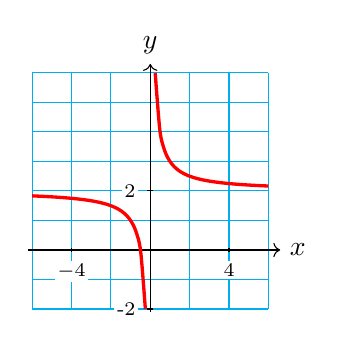
\begin{tikzpicture} [xscale=.5, yscale=.375]
\draw[cyan] (-3,-2) grid (3,6);

\draw[->] (-3.1,0) -- (3.3,0) node[right] {$x$};
\draw[->] (0,-2.1) -- (0,6.3) node[above] {$y$};

\foreach \x [evaluate=\x as \xi using int( 2* \x )] in {-2,2} \draw[black] ($ \x *(1,0) +(0,.08) $) --++(0,-.16) node[anchor=north, xshift=0,yshift=-3, fill=white, inner sep=1pt] {\scriptsize$ \xi $};

\foreach \y [evaluate=\y as \yi using int( 1* \y )]   in {-2, 2} \draw[black] (.08,\y ) --++(-.16,0) node[anchor=east, xshift=-3, fill=white, inner sep=1pt] {\scriptsize\yi};

\draw[domain={-3:-1/8},smooth,variable=\x,red,very thick] plot ({\x},{ (4*\x+1)/( 2*\x ) });

\draw[domain={1/8:3},smooth,variable=\x,red,very thick] plot ({\x},{ (4*\x+1)/( 2*\x )});

\end{tikzpicture}
\newline


ar4-3-6ans $f(x) = \frac{x}{ x-1 }$
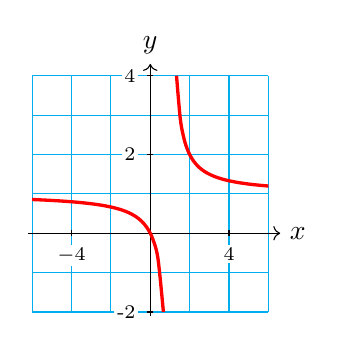
\begin{tikzpicture} [scale=.5]
\draw[cyan] (-3,-2) grid (3,4);

\draw[->] (-3.1,0) -- (3.3,0) node[right] {$x$};
\draw[->] (0,-2.1) -- (0,4.3) node[above] {$y$};

\foreach \x [evaluate=\x as \xi using int( 2* \x )] in {-2,2} \draw[black] ($ \x *(1,0) +(0,.08) $) --++(0,-.16) node[anchor=north, xshift=0,yshift=-3, fill=white, inner sep=1pt] {\scriptsize$ \xi $};

\foreach \y [evaluate=\y as \yi using int( 1* \y )]   in {-2, 2, 4} \draw[black] (.08,\y ) --++(-.16,0) node[anchor=east, xshift=-3, fill=white, inner sep=1pt] {\scriptsize\yi};

\draw[domain={-3:1/3},smooth,variable=\x,red,very thick] plot ({\x},{ (2*\x)/( 2*\x - 1) });

\draw[domain={4/6:3},smooth,variable=\x,red,very thick] plot ({\x},{ (2*\x)/( 2*\x - 1 )});

\end{tikzpicture}
\newline



hp4-2-59ans tangent graph

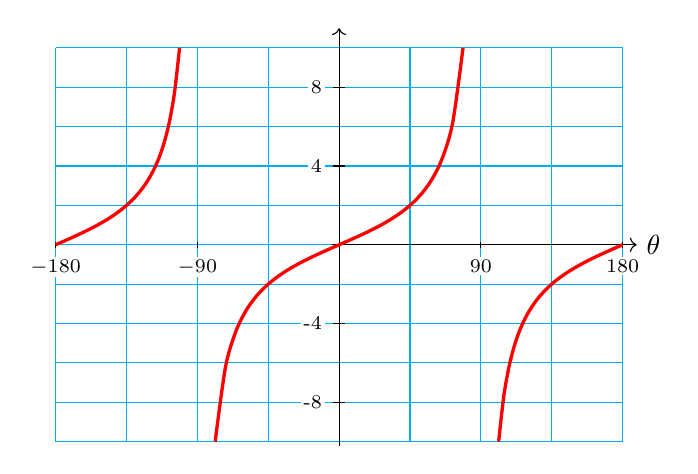
\begin{tikzpicture} [xscale=.9,yscale=.5]
\draw[cyan] (-4,-5) grid (4,5);

\draw[->] (-.1,0) -- (4.2,0) node[right] {$\theta$};
\draw[->] (0,-5.1) -- (0,5.5);
\foreach \x [evaluate=\x as \xi using int( 45* \x )] in {-4, -2, 2, 4} \draw[black] ($ \x *(1,0) +(0,.08) $) --++(0,-.16) node[anchor=north, xshift=0,yshift=-3, fill=white, inner sep=1pt] {\scriptsize$ \xi $};

\foreach \y [evaluate=\y as \yi using int( 2* \y )]   in {-4,-2, 2,4} \draw[black] (.08,\y ) --++(-.16,0) node[anchor=east, xshift=-3, fill=white, inner sep=1pt] {\scriptsize\yi};

\draw[domain={atan(-5)/45:atan(5)/45},smooth,variable=\x,red,very thick] plot ({\x},{tan(45*\x)});

\draw[domain={atan(-5)/45+4:4},smooth,variable=\x,red,very thick] plot ({\x},{tan(45*\x)});

\draw[domain={-4:atan(5)/45-4},smooth,variable=\x,red,very thick] plot ({\x},{tan(45*\x)});

\end{tikzpicture}
\newline


\section{4.3 homework}


hp4-3-1 grid
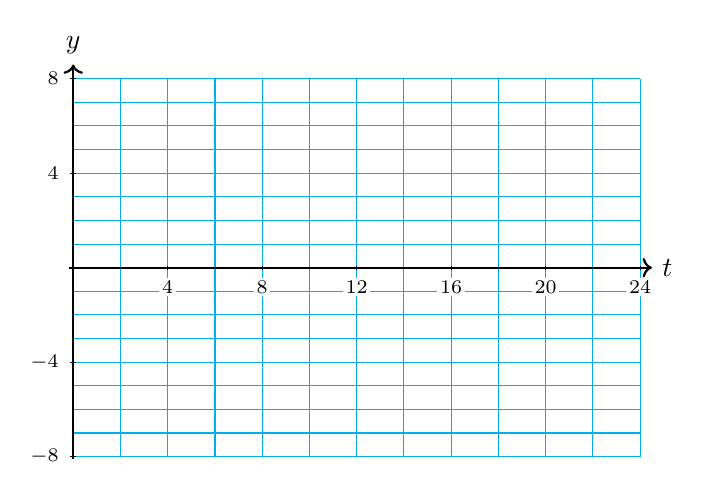
\begin{tikzpicture} [scale=.3]
\draw[cyan, xstep=2, ystep=1] (0,-8) grid (24,8);

\draw[black,thick, ->] (-.2,0) -- (24.5,0) node[right]{$t$};
\draw[black, thick, ->] (0,-8.1) -- (0,8.6) node[above]{$y$};

\foreach \x in {4, 8, ..., 24} 
  \draw[black] ($ \x *(1,0) +(0,.08) $) --++(0,-.16) node[anchor=north, xshift=0,yshift=-3, fill=white, inner sep=1pt] {\scriptsize$ \x $};
\foreach \y in {-8, -4, 4, 8} 
  \draw[black] ($ \y *(0,1) +(.12,0) $) --++(-.24,0) node[anchor=east, xshift=-3, fill=white, inner sep=1pt] {\scriptsize$ \y $};

\end{tikzpicture}
\newline

hp4-3-1ansa sundial on grid
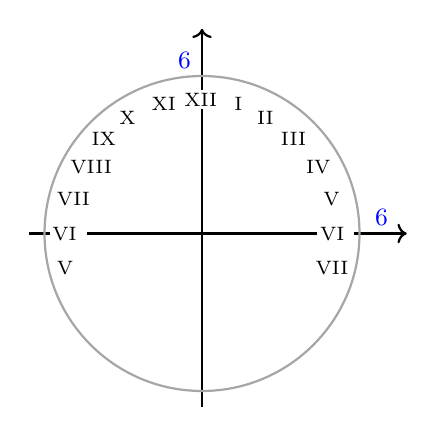
\begin{tikzpicture} 
\draw[black,thick, ->] (-2.2,0) -- +(4.8,0);
\draw[black, thick, ->] (0,-2.2) -- +(0,4.8);

\coordinate (O) at (0,0);
\draw[gray!70, thick] (O) circle (2cm);
\node[anchor=center, text width=.2, xshift=-.3cm, text=blue] at (90:2.2){\small 6};
\node[anchor=center, text width=.1, yshift=.2cm, text=blue] at (0:2.2){\small 6};
\node[text width=.45cm,fill=white, inner sep=1pt] at (90:1.7){\scriptsize XII};
\node[ text width=.2cm, xshift=2] at (75:1.7){\scriptsize I};
\node[ text width=.3cm] at (60:1.7){\scriptsize II};
\node[ text width=.4cm] at (45:1.7){\scriptsize III};
\node[ text width=.3cm] at (30:1.7){\scriptsize IV};
\node[ text width=.2cm] at (15:1.7){\scriptsize V};
\node[ text width=.4cm, fill=white, inner sep=1pt] at (0:1.7){\scriptsize VI};
\node[ text width=.4cm] at (-15:1.7){\scriptsize VII};

\node[ text width=.4cm] at (105:1.7){\scriptsize XI};
\node[ text width=.4cm] at (120:1.7){\scriptsize X};
\node[ text width=.4cm] at (135:1.7){\scriptsize IX};
\node[ text width=.4cm] at (150:1.7){\scriptsize VIII};
\node[ text width=.4cm] at (165:1.7){\scriptsize VII};
\node[anchor=center, text width=.4cm, fill=white, inner sep=1pt] at (180:1.7){\scriptsize VI};
\node[ text width=.4cm] at (195:1.7){\scriptsize V};

\end{tikzpicture}
\newline

hp4-3-1ansc sinusoidal graph
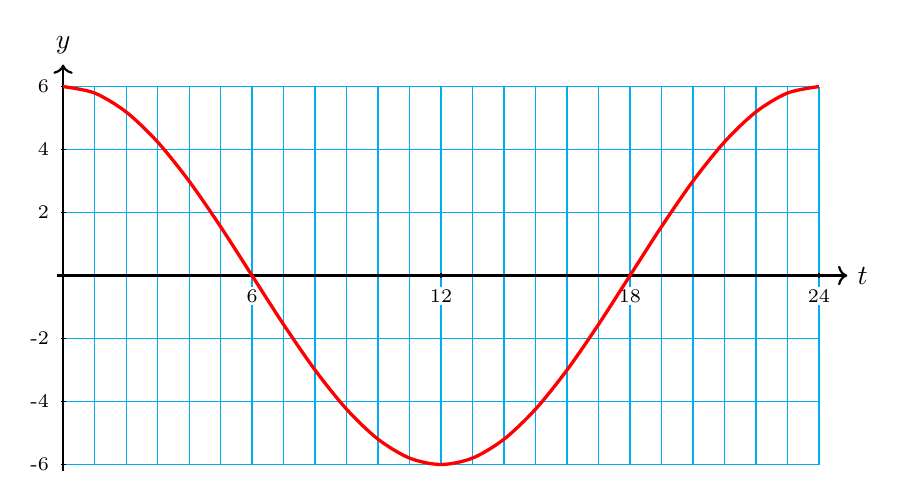
\begin{tikzpicture} [scale=.4]
\draw[cyan, ystep=2] (0,-6) grid (24,6);
\draw[black, thick, ->] (-.2,0) -- (24.9,0) node[anchor=west]{$t$};
\draw[black, thick, ->] (0, -6.2) -- (0, 6.7) node[anchor=south] {$y$};

\foreach \x in {6, 12, 18, 24} \draw[black] ($ \x *(1,0) +(0,.08) $) --++(0,-.16) node[anchor=north, xshift=0,yshift=-3, fill=white, inner sep=1pt] {\scriptsize$ \x $};

\foreach \y   in {-6, -4,-2, 2,4,6} \draw[black] (.08,\y ) --++(-.16,0) node[anchor=east, xshift=-3, fill=white, inner sep=1pt] {\scriptsize\y};

\draw[domain=0:24,smooth,variable=\x,red,very thick] plot ({\x},{6*cos(15*\x)});

\end{tikzpicture}
\newline

hp4-3-3 square on grid
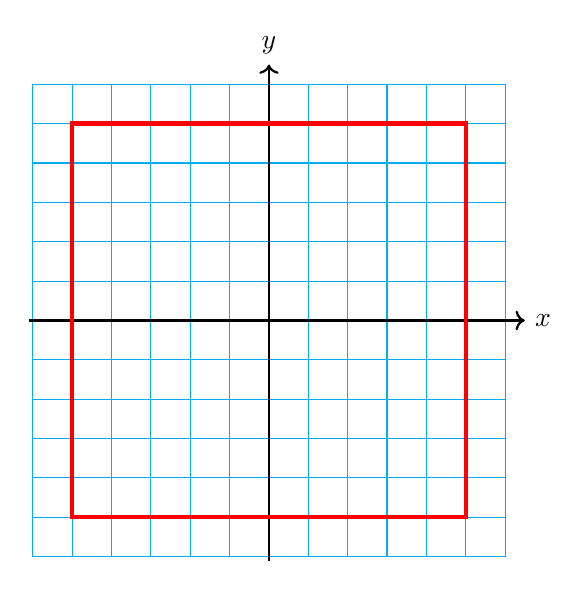
\begin{tikzpicture} [scale=0.5]
\draw[cyan] (-6,-6) grid (6,6);
\draw[black, thick, ->] (-6.1,0)--(6.5,0) node[right]{$x$};
\draw[black, thick, ->] (0, -6.1)--(0, 6.5) node[above]{$y$};

\draw[red, ultra thick] (-5,-5) rectangle (5,5);

\end{tikzpicture}
\newline

hp4-3-3b grid
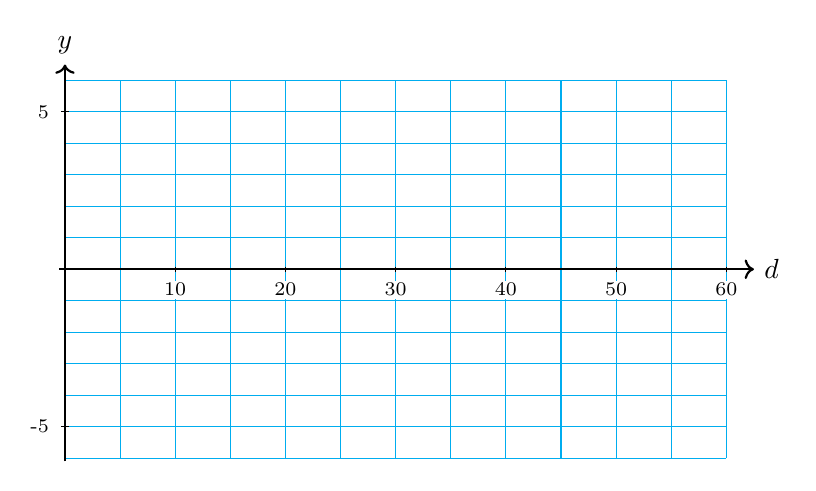
\begin{tikzpicture} [xscale=0.7, yscale=.4]
\draw[cyan] (0,-6) grid (12,6);
\draw[black, thick, ->] (-0.1,0)--(12.5,0) node[right]{$d$};
\draw[black, thick, ->] (0, -6.1)--(0, 6.5) node[above]{$y$};

\foreach \x [evaluate=\x as \xi using int( 5* \x )] in { 2, 4, ..., 12} \draw[black] ($ \x *(1,0) +(0,.08) $) --++(0,-.16) node[anchor=north, xshift=0,yshift=-3, fill=white, inner sep=1pt] {\scriptsize$ \xi $};

\foreach \y   in { -5, 5} \draw[black] (.08,\y ) --++(-.16,0) node[anchor=east, xshift=-3, fill=white, inner sep=1pt] {\scriptsize\y};
\end{tikzpicture}
\newline

hp4-3-3ans periodic function
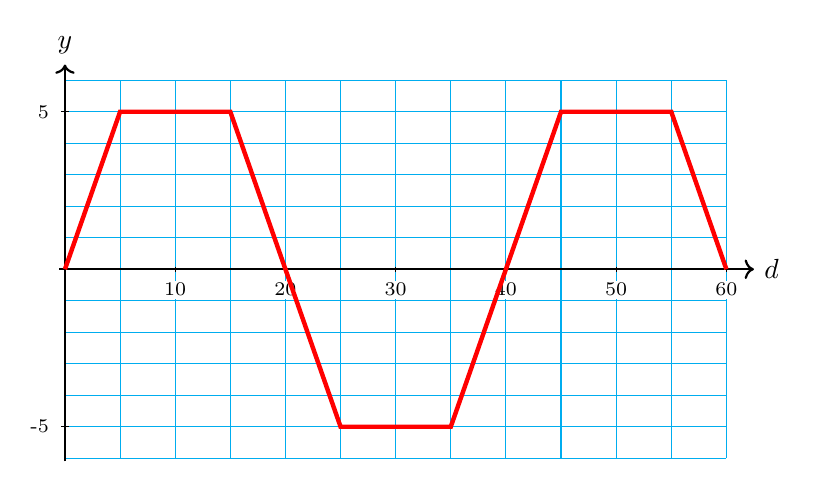
\begin{tikzpicture} [xscale=0.7, yscale=.4]
\draw[cyan] (0,-6) grid (12,6);
\draw[black, thick, ->] (-0.1,0)--(12.5,0) node[right]{$d$};
\draw[black, thick, ->] (0, -6.1)--(0, 6.5) node[above]{$y$};

\foreach \x [evaluate=\x as \xi using int( 5* \x )] in { 2, 4, ..., 12} \draw[black] ($ \x *(1,0) +(0,.08) $) --++(0,-.16) node[anchor=north, xshift=0,yshift=-3, fill=white, inner sep=1pt] {\scriptsize$ \xi $};

\foreach \y   in { -5, 5} \draw[black] (.08,\y ) --++(-.16,0) node[anchor=east, xshift=-3, fill=white, inner sep=1pt] {\scriptsize\y};

\draw[red, ultra thick] (0,0)--(1,5)--(3,5)--(5,-5) -- (7,-5) -- (9,5) -- (11,5) -- (12,0);

\end{tikzpicture}
\newline

hp4-3-13 grid
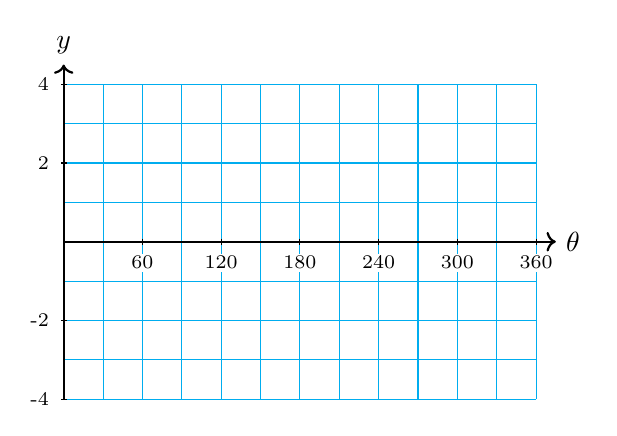
\begin{tikzpicture} [scale=.5]
\draw[cyan] (0,-4) grid (12,4);
\draw[black, thick, ->] (0,0)--(12.5,0) node[right]{$\theta$};
\draw[black, thick, ->] (0,-4)--(0,4.5) node[above]{$y$};

\foreach \x [evaluate=\x as \xi using int( 30* \x )] in { 2, 4, ..., 12} \draw[black] ($ \x *(1,0) +(0,.08) $) --++(0,-.16) node[anchor=north, xshift=0,yshift=-3, fill=white, inner sep=1pt] {\scriptsize$ \xi $};

\foreach \y   in { -4, -2, 2, 4} \draw[black] (.08,\y ) --++(-.16,0) node[anchor=east, xshift=-3, fill=white, inner sep=1pt] {\scriptsize\y};

\end{tikzpicture}
\newline

hp4-3-13ans 3 cos theta
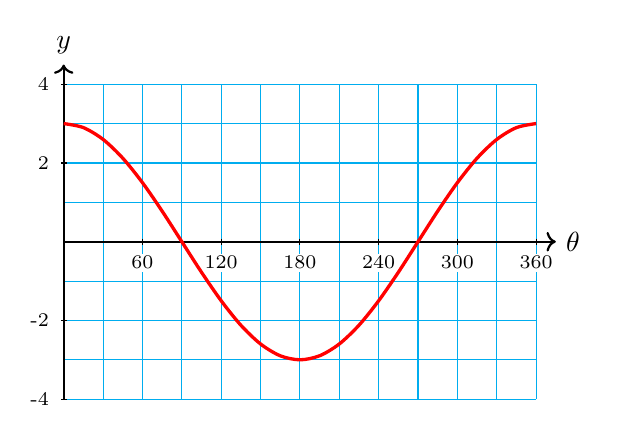
\begin{tikzpicture} [scale=.5]
\draw[cyan] (0,-4) grid (12,4);
\draw[black, thick, ->] (0,0)--(12.5,0) node[right]{$\theta$};
\draw[black, thick, ->] (0,-4)--(0,4.5) node[above]{$y$};

\foreach \x [evaluate=\x as \xi using int( 30* \x )] in { 2, 4, ..., 12} \draw[black] ($ \x *(1,0) +(0,.08) $) --++(0,-.16) node[anchor=north, xshift=0,yshift=-3, fill=white, inner sep=1pt] {\scriptsize$ \xi $};

\foreach \y   in { -4, -2, 2, 4} \draw[black] (.08,\y ) --++(-.16,0) node[anchor=east, xshift=-3, fill=white, inner sep=1pt] {\scriptsize\y};

\draw[domain={0:12},smooth,variable=\x,red,very thick] plot ({\x},{3*cos(30*\x)});

\end{tikzpicture}
\newline

hp4-3-15ans $y = 3 + \sin \theta$
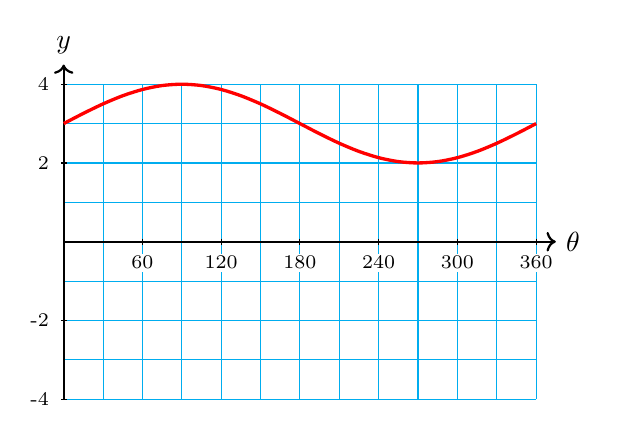
\begin{tikzpicture} [scale=.5]
\draw[cyan] (0,-4) grid (12,4);
\draw[black, thick, ->] (0,0)--(12.5,0) node[right]{$\theta$};
\draw[black, thick, ->] (0,-4)--(0,4.5) node[above]{$y$};

\foreach \x [evaluate=\x as \xi using int( 30* \x )] in { 2, 4, ..., 12} \draw[black] ($ \x *(1,0) +(0,.08) $) --++(0,-.16) node[anchor=north, xshift=0,yshift=-3, fill=white, inner sep=1pt] {\scriptsize$ \xi $};

\foreach \y   in { -4, -2, 2, 4} \draw[black] (.08,\y ) --++(-.16,0) node[anchor=east, xshift=-3, fill=white, inner sep=1pt] {\scriptsize\y};

\draw[domain={0:12},smooth,variable=\x,red,very thick] plot ({\x},{3 + sin(30*\x)});

\end{tikzpicture}
\newline

hp4-3-17ans $y = \cos 3 \theta$
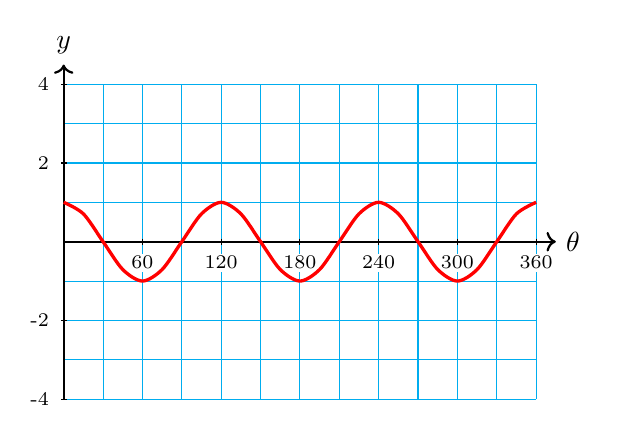
\begin{tikzpicture} [scale=.5]
\draw[cyan] (0,-4) grid (12,4);
\draw[black, thick, ->] (0,0)--(12.5,0) node[right]{$\theta$};
\draw[black, thick, ->] (0,-4)--(0,4.5) node[above]{$y$};

\foreach \x [evaluate=\x as \xi using int( 30* \x )] in { 2, 4, ..., 12} \draw[black] ($ \x *(1,0) +(0,.08) $) --++(0,-.16) node[anchor=north, xshift=0,yshift=-3, fill=white, inner sep=1pt] {\scriptsize$ \xi $};

\foreach \y   in { -4, -2, 2, 4} \draw[black] (.08,\y ) --++(-.16,0) node[anchor=east, xshift=-3, fill=white, inner sep=1pt] {\scriptsize\y};

\draw[domain={0:12},smooth,variable=\x,red,very thick] plot ({\x},{cos(90*\x)});

\end{tikzpicture}
\newline


hp4-3-25 $y = \sin 4 \theta$
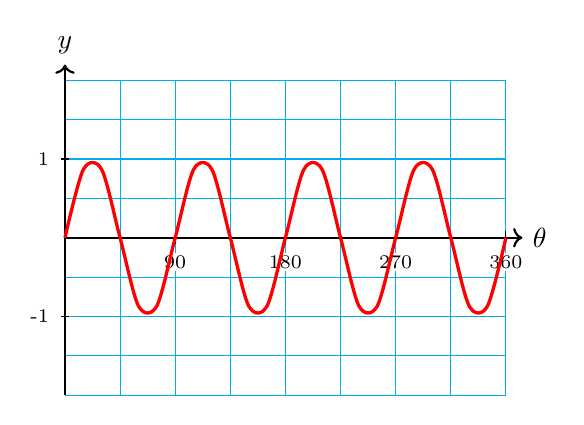
\begin{tikzpicture} [xscale=.7, yscale=1]
\draw[cyan, xstep=1, ystep=1/2] (0,-2) grid (8,2);
\draw[black, thick, ->] (0,0)--(8.3,0) node[right]{$\theta$};
\draw[black, thick, ->] (0,-2)--(0,2.2) node[above]{$y$};

\foreach \x [evaluate=\x as \xi using int( 45* \x )] in { 2, 4, ..., 8} \draw[black] ($ \x *(1,0) +(0,.08) $) --++(0,-.16) node[anchor=north, xshift=0,yshift=-3, fill=white, inner sep=1pt] {\scriptsize$ \xi $};

\foreach \y   in { -1,1} \draw[black] (.08,\y ) --++(-.16,0) node[anchor=east, xshift=-3, fill=white, inner sep=1pt] {\scriptsize\y};

\draw[domain={0:8},smooth,variable=\x,red,very thick] plot ({\x},{sin(4*45*\x)});

\end{tikzpicture}
\newline


hp4-3-26 $y = 4 \sin \theta$
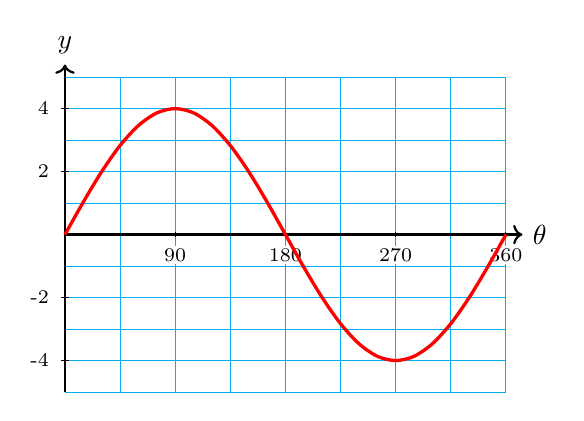
\begin{tikzpicture} [xscale=.7, yscale=.4]
\draw[cyan ] (0,-5) grid (8,5);
\draw[black, thick, ->] (0,0)--(8.3,0) node[right]{$\theta$};
\draw[black, thick, ->] (0,-5)--(0,5.4) node[above]{$y$};

\foreach \x [evaluate=\x as \xi using int( 45* \x )] in { 2, 4, ..., 8} \draw[black] ($ \x *(1,0) +(0,.08) $) --++(0,-.16) node[anchor=north, xshift=0,yshift=-3, fill=white, inner sep=1pt] {\scriptsize$ \xi $};

\foreach \y   in { -4, -2, 2, 4} \draw[black] (.08,\y ) --++(-.16,0) node[anchor=east, xshift=-3, fill=white, inner sep=1pt] {\scriptsize\y};

\draw[domain={0:8},smooth,variable=\x,red,very thick] plot ({\x},{4*sin(45*\x)});

\end{tikzpicture}
\newline


hp4-3-27 $y = 3+ \cos \theta$
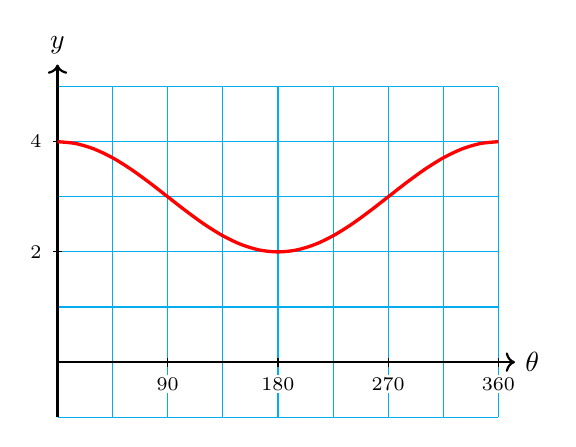
\begin{tikzpicture} [xscale=.7, yscale=.7]
\draw[cyan ] (0,-1) grid (8,5);
\draw[black, thick, ->] (0,0)--(8.3,0) node[right]{$\theta$};
\draw[black, thick, ->] (0,-1)--(0,5.4) node[above]{$y$};

\foreach \x [evaluate=\x as \xi using int( 45* \x )] in { 2, 4, ..., 8} \draw[black] ($ \x *(1,0) +(0,.08) $) --++(0,-.16) node[anchor=north, xshift=0,yshift=-3, fill=white, inner sep=1pt] {\scriptsize$ \xi $};

\foreach \y   in { 2, 4} \draw[black] (.08,\y ) --++(-.16,0) node[anchor=east, xshift=-3, fill=white, inner sep=1pt] {\scriptsize\y};

\draw[domain={0:8},smooth,variable=\x,red,very thick] plot ({\x},{3+cos(45*\x)});

\end{tikzpicture}
\newline


hp4-3-28 $y = 3 \cos \theta$
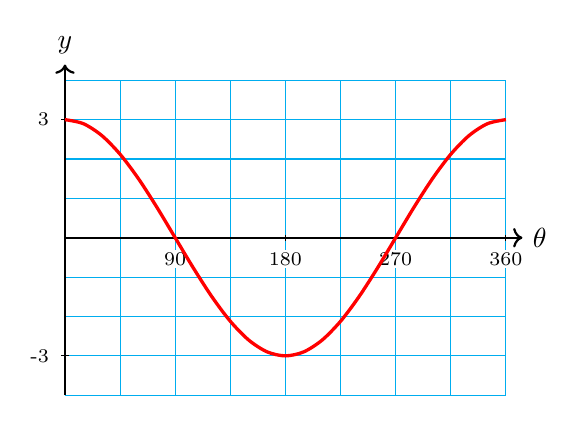
\begin{tikzpicture} [xscale=.7, yscale=.5]
\draw[cyan ] (0,-4) grid (8,4);
\draw[black, thick, ->] (0,0)--(8.3,0) node[right]{$\theta$};
\draw[black, thick, ->] (0,-4)--(0,4.4) node[above]{$y$};

\foreach \x [evaluate=\x as \xi using int( 45* \x )] in { 2, 4, ..., 8} \draw[black] ($ \x *(1,0) +(0,.08) $) --++(0,-.16) node[anchor=north, xshift=0,yshift=-3, fill=white, inner sep=1pt] {\scriptsize$ \xi $};

\foreach \y   in { -3,3} \draw[black] (.08,\y ) --++(-.16,0) node[anchor=east, xshift=-3, fill=white, inner sep=1pt] {\scriptsize\y};

\draw[domain={0:8},smooth,variable=\x,red,very thick] plot ({\x},{3*cos(45*\x)});

\end{tikzpicture}
\newline


hp4-3-29 $y = -2+ 4* \sin \theta$
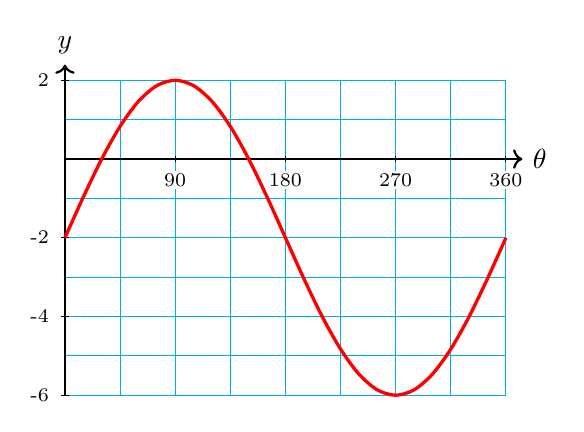
\begin{tikzpicture} [xscale=.7, yscale=.5]
\draw[cyan ] (0,-6) grid (8,2);
\draw[black, thick, ->] (0,0)--(8.3,0) node[right]{$\theta$};
\draw[black, thick, ->] (0,-6)--(0,2.4) node[above]{$y$};

\foreach \x [evaluate=\x as \xi using int( 45* \x )] in { 2, 4, ..., 8} \draw[black] ($ \x *(1,0) +(0,.08) $) --++(0,-.16) node[anchor=north, xshift=0,yshift=-3, fill=white, inner sep=1pt] {\scriptsize$ \xi $};

\foreach \y   in { -6, -4, -2, 2} \draw[black] (.08,\y ) --++(-.16,0) node[anchor=east, xshift=-3, fill=white, inner sep=1pt] {\scriptsize\y};

\draw[domain={0:8},smooth,variable=\x,red,very thick] plot ({\x},{-2+4*sin(45*\x)});

\end{tikzpicture}
\newline


hp4-3-30 $y = -2+  \cos 4 \theta$
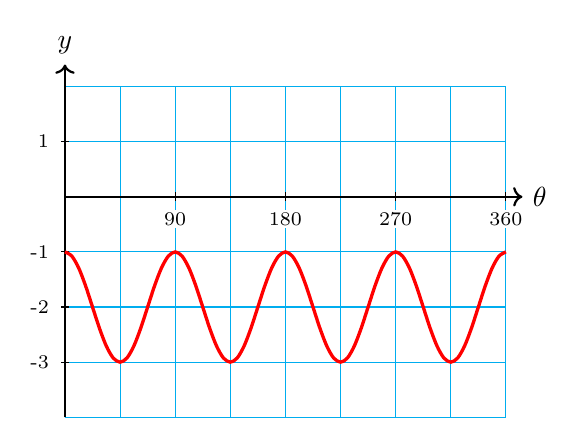
\begin{tikzpicture} [xscale=.7, yscale=.7]
\draw[cyan ] (0,-4) grid (8,2);
\draw[black, thick, ->] (0,0)--(8.3,0) node[right]{$\theta$};
\draw[black, thick, ->] (0,-4)--(0,2.4) node[above]{$y$};

\foreach \x [evaluate=\x as \xi using int( 45* \x )] in { 2, 4, ..., 8} \draw[black] ($ \x *(1,0) +(0,.08) $) --++(0,-.16) node[anchor=north, xshift=0,yshift=-3, fill=white, inner sep=1pt] {\scriptsize$ \xi $};

\foreach \y   in { -3, -2, -1,1} \draw[black] (.08,\y ) --++(-.16,0) node[anchor=east, xshift=-3, fill=white, inner sep=1pt] {\scriptsize\y};

\draw[samples=65,domain={0:8},smooth,variable=\x,red,very thick] plot ({\x},{-2+cos(4*45*\x)});

\end{tikzpicture}
\newline


hp4-3-31 $y = 2+  2 \cos 3 \theta$
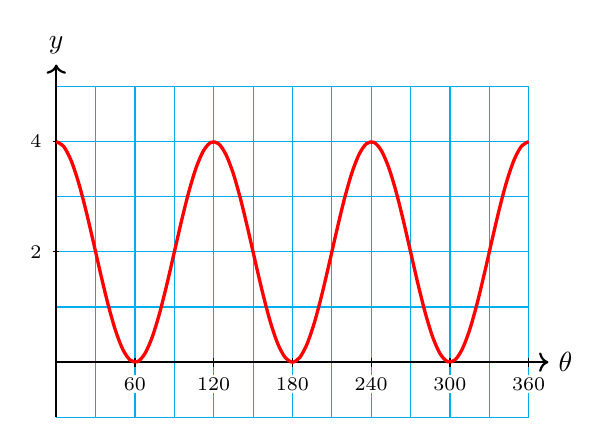
\begin{tikzpicture} [xscale=.5, yscale=.7]
\draw[cyan ] (0,-1) grid (12,5);
\draw[black, thick, ->] (0,0)--(12.5,0) node[right]{$\theta$};
\draw[black, thick, ->] (0,-1)--(0,5.4) node[above]{$y$};

\foreach \x [evaluate=\x as \xi using int( 30* \x )] in { 2, 4, ..., 12} \draw[black] ($ \x *(1,0) +(0,.08) $) --++(0,-.16) node[anchor=north, xshift=0,yshift=-3, fill=white, inner sep=1pt] {\scriptsize$ \xi $};

\foreach \y   in { 2,4} \draw[black] (.08,\y ) --++(-.16,0) node[anchor=east, xshift=-3, fill=white, inner sep=1pt] {\scriptsize\y};

\draw[samples=65,domain={0:12},smooth,variable=\x,red,very thick] plot ({\x},{2+2*cos(3*30*\x)});

\end{tikzpicture}
\newline


hp4-3-32 $y = -1+  4 \sin 3 \theta$
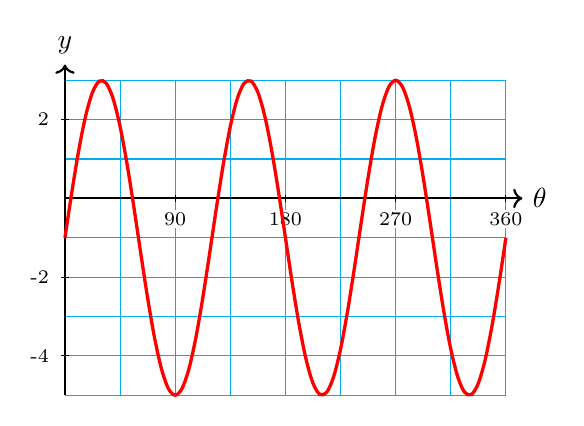
\begin{tikzpicture} [xscale=.7, yscale=.5]
\draw[cyan ] (0,-5) grid (8,3);
\draw[black, thick, ->] (0,0)--(8.3,0) node[right]{$\theta$};
\draw[black, thick, ->] (0,-5)--(0,3.4) node[above]{$y$};

\foreach \x [evaluate=\x as \xi using int( 45* \x )] in { 2, 4, ..., 8} \draw[black] ($ \x *(1,0) +(0,.08) $) --++(0,-.16) node[anchor=north, xshift=0,yshift=-3, fill=white, inner sep=1pt] {\scriptsize$ \xi $};

\foreach \y   in { -4, -2, 2} \draw[black] (.08,\y ) --++(-.16,0) node[anchor=east, xshift=-3, fill=white, inner sep=1pt] {\scriptsize\y};

\draw[samples=65,domain={0:8},smooth,variable=\x,red,very thick] plot ({\x},{-1+4*sin(3*45*\x)});

\end{tikzpicture}
\newline


hp4-3-43 $y = -3 \cos  \theta$
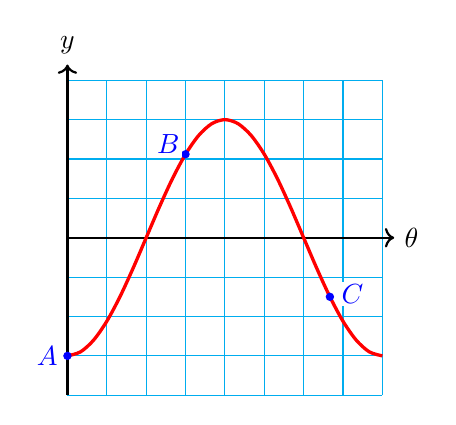
\begin{tikzpicture} [scale=.5]
\draw[cyan, xstep=1 ] (0,-4) grid (8,4);
\draw[black, thick, ->] (0,0)--(8.3,0) node[right]{$\theta$};
\draw[black, thick, ->] (0,-4)--(0,4.4) node[above]{$y$};

\draw[domain={0:8},smooth,variable=\x,red,very thick] plot ({\x},{-3*cos(45*\x)});

\coordinate (A) at (0,-3);
\coordinate (B) at ($(3,0) + 3*cos(135)*(0,-1) $);
\coordinate (C) at ($ (20/3,0) +3*cos(300)*(0,-1)$);

\filldraw[blue] (A) circle (2.6pt) node[anchor=east]{$A$};
\filldraw[blue] (B) circle (2.6pt) node[anchor=south east, xshift=-1, yshift=-1, fill=white, inner sep=1pt]{$B$};
\filldraw[blue] (C) circle (2.6pt) node[anchor=west, xshift=3, yshift=1, fill=white, inner sep=1pt]{$C$};

\end{tikzpicture}
\newline


hp4-3-44 $y = 4 \sin  \theta$
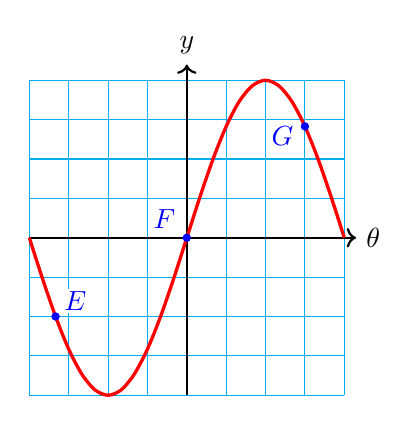
\begin{tikzpicture} [scale=.5]
\draw[cyan, xstep=1 ] (-4,-4) grid (4,4);
\draw[black, thick, ->] (-4,0)--(4.3,0) node[right]{$\theta$};
\draw[black, thick, ->] (0,-4)--(0,4.4) node[above]{$y$};

\draw[domain={-4:4},smooth,variable=\x,red,very thick] plot ({\x},{4*sin(45*\x)});

\coordinate (A) at ($(-10/3,0) + 4*sin(-150)*(0,1) $);
\coordinate (B) at (0,0);
\coordinate (C) at ($ (3,0) +4*sin(135)*(0,1)$);

\filldraw[blue] (A) circle (2.6pt) node[anchor=south west, xshift=2, yshift=1, fill=white, inner sep=1pt]{$E$};
\filldraw[blue] (B) circle (2.6pt) node[anchor=south east, xshift=-3, yshift=2, fill=white, inner sep=1pt]{$F$};
\filldraw[blue] (C) circle (2.6pt) node[anchor=north east, xshift=-3, yshift=1, fill=white, inner sep=1pt]{$G$};

\end{tikzpicture}
\newline


hp4-3-45 $y = \sin 4 \theta$
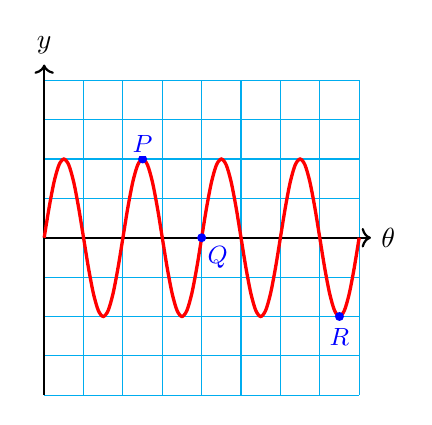
\begin{tikzpicture} [scale=.5]
\draw[cyan, xstep=1 ] (-0,-4) grid (8,4);
\draw[black, thick, ->] (0,0)--(8.3,0) node[right]{$\theta$};
\draw[black, thick, ->] (0,-4)--(0,4.4) node[above]{$y$};

\draw[samples=65,domain={-0:8},smooth,variable=\x,red,very thick] plot ({\x},{2*sin(4* 45*\x)});

\coordinate (A) at ($(2.5,0) + 2*sin(450)*(0,1) $);
\coordinate (B) at (4,0);
\coordinate (C) at ($ (7.5,0) +2*sin(1350)*(0,1)$);

\filldraw[blue] (A) circle (2.8pt) node[anchor=south, xshift=0, yshift=1, fill=white, inner sep=1pt]{\small $P$};
\filldraw[blue] (B) circle (2.8pt) node[anchor=north west, xshift=1, yshift=-2, fill=white, inner sep=1pt]{\small $Q$};
\filldraw[blue] (C) circle (2.8pt) node[anchor=north , xshift=0, yshift=-3, fill=white, inner sep=1pt]{\small $R$};

\end{tikzpicture}
\newline


hp4-3-46 $y = \cos 3 \theta$
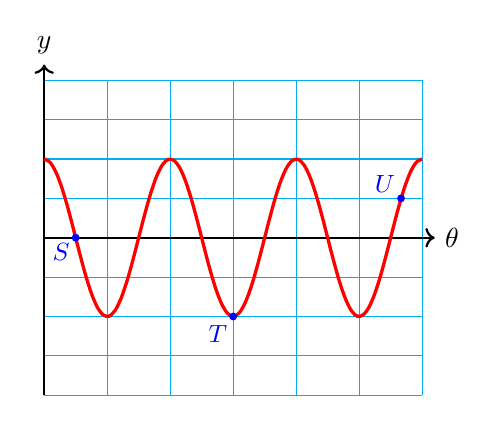
\begin{tikzpicture} [xscale=.4, yscale=.5]
\draw[cyan, xstep=2 ] (-0,-4) grid (12,4);
\draw[black, thick, ->] (0,0)--(12.4,0) node[right]{$\theta$};
\draw[black, thick, ->] (0,-4)--(0,4.4) node[above]{$y$};

\draw[samples=65,domain={-0:12},smooth,variable=\x,red,very thick] plot ({\x},{2*cos(3* 30*\x)});

\coordinate (A) at ($(1,0) + 2*cos(90)*(0,1) $);
\coordinate (B) at (6,-2);
\coordinate (C) at ($ (11.33,0) +2*cos(1020)*(0,1)$);

\filldraw[blue] (A) ellipse (3pt and 2.4pt) node[anchor=north east, xshift=-1, yshift=-1, fill=white, inner sep=1pt]{\small $S$};
\filldraw[blue] (B) ellipse (3pt and 2.4pt) node[anchor=north east, xshift=-1, yshift=-2, fill=white, inner sep=1pt]{\small $T$};
\filldraw[blue] (C) ellipse (3pt and 2.4pt) node[anchor=south east , xshift=-1, yshift=1, fill=white, inner sep=1pt]{\small $U$};

\end{tikzpicture}
\newline


hp4-3-47 $y = -3 + \cos \theta$
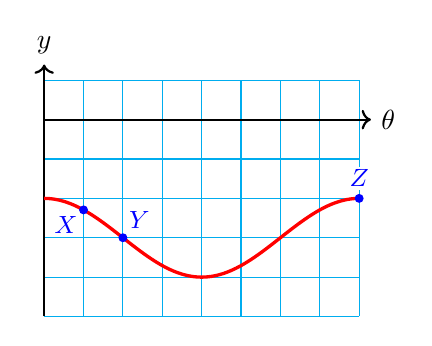
\begin{tikzpicture} [scale=.5]
\draw[cyan, xstep=1 ] (-0,-5) grid (8,1);
\draw[black, thick, ->] (0,0)--(8.3,0) node[right]{$\theta$};
\draw[black, thick, ->] (0,-5)--(0,1.4) node[above]{$y$};

\draw[samples=65,domain={-0:8},smooth,variable=\x,red,very thick] plot ({\x},{-3 + cos( 45*\x)});

\coordinate (A) at ($(1,-3) + cos(45)*(0,1) $);
\coordinate (B) at (2,-3);
\coordinate (C) at (8,-2);

\filldraw[blue] (A) circle (2.8pt) node[anchor=north east, xshift=-1, yshift=-1, fill=white, inner sep=1pt]{\small $X$};
\filldraw[blue] (B) circle (2.8pt) node[anchor=south west, xshift=1, yshift=2, fill=white, inner sep=1pt]{\small $Y$};
\filldraw[blue] (C) circle (2.8pt) node[anchor=south , xshift=0, yshift=3, fill=white, inner sep=1pt]{\small $Z$};

\end{tikzpicture}
\newline


hp4-3-48 $y = 1 +\sin  \theta$
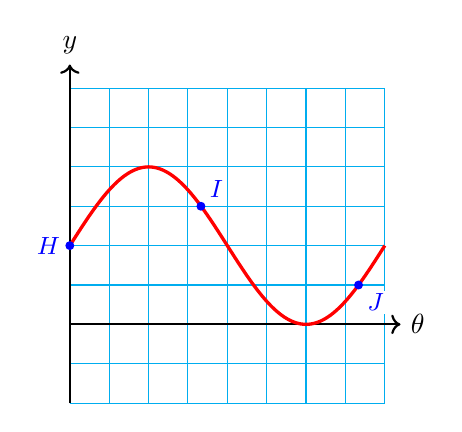
\begin{tikzpicture} [scale=.5]
\draw[cyan, xstep=1 ] (-0,-2) grid (8,6);
\draw[black, thick, ->] (0,0)--(8.4,0) node[right]{$\theta$};
\draw[black, thick, ->] (0,-2)--(0,6.6) node[above]{$y$};

\draw[samples=65,domain={-0:8},smooth,variable=\x,red,very thick] plot ({\x},{2+ 2*sin( 45*\x)});

\coordinate (A) at (0, 2);
\coordinate (B) at (3.33, 3);
\coordinate (C) at (7.333, 1);

\filldraw[blue] (A) circle (2.8pt) node[anchor=east]{\small $H$};
\filldraw[blue] (B) circle (2.8pt) node[anchor=south west, xshift=2, yshift=2, fill=white, inner sep=1pt]{\small $I$};
\filldraw[blue] (C) circle (2.8pt) node[anchor=north west, xshift=2, yshift=-2, fill=white, inner sep=1pt]{\small $J$};

\end{tikzpicture}
\newline


hp4-3-53ans piecewise linear periodic
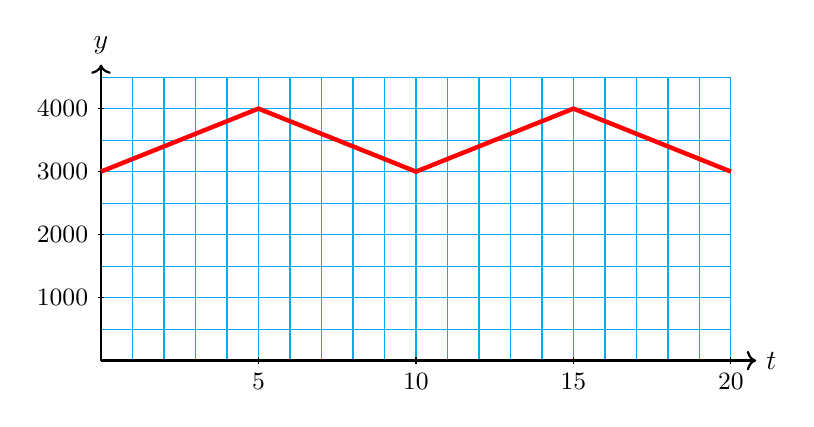
\begin{tikzpicture} [scale=.4]

\draw[cyan] (0,0) grid (20,9);
\draw[black,thick,->] (0,0) --(20.8,0) node[right]{$t$};
\draw[black,thick,->] (0,0) --(0,9.4) node[above]{$y$};

\foreach \x in {5, 10, 15, 20} {
 \draw[black] (\x,0.1)--+(0, -.2) node[below]{\small \x};
};
\foreach \y [evaluate=\y as \yi using int( 500* \y )] in {2, 4, 6, 8} {
 \draw[black] (0.1,\y)--+(-.2,0) node[left]{\small \yi};
};

\draw[red, ultra thick] (0,6)--++(5,2)--++(5,-2) --++(5,2)--++(5,-2);
\end{tikzpicture}
\newline


hp4-3-55ans piecewise linear periodic
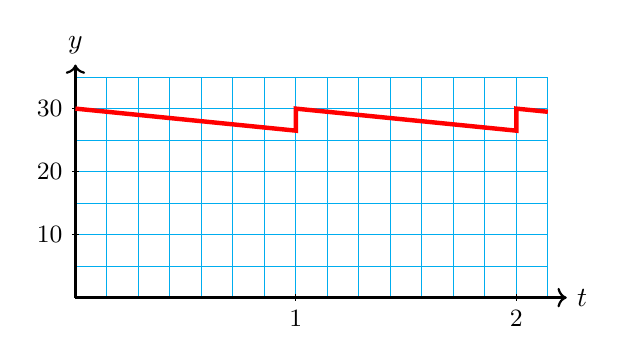
\begin{tikzpicture} [scale=.4]

\draw[cyan] (0,0) grid (15,7);
\draw[black,thick,->] (0,0) --(15.6,0) node[right]{$t$};
\draw[black,thick,->] (0,0) --(0,7.4) node[above]{$y$};

\foreach \x [evaluate=\x as \xi using int( \x/7)] in {7, 14} {
 \draw[black] (\x,0.1)--+(0, -.2) node[below]{\small \xi};
};
\foreach \y [evaluate=\y as \yi using int( 5* \y )] in {2, 4, 6} {
 \draw[black] (0.1,\y)--+(-.2,0) node[left]{\small \yi};
};

\draw[red, ultra thick] (0,6)--++(7,-.7)--++(0,.7) --++(7,-.7)--++(0,.7)--++(1, -.1);
\end{tikzpicture}
\newline



hp4-3-57ans sinusoidal $y=12+10\cos 2\pi t$

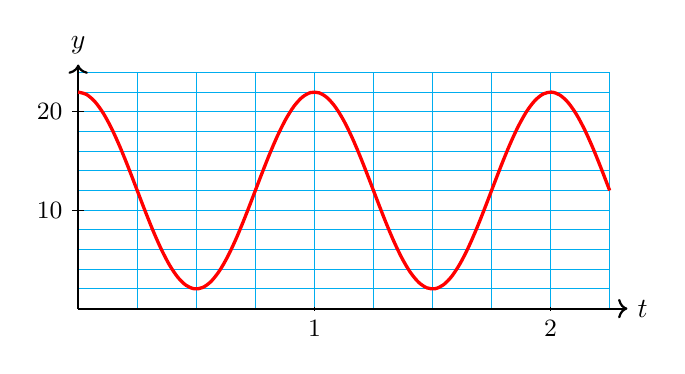
\begin{tikzpicture} [xscale=.75, yscale=.25]

\draw[cyan] (0,0) grid (9,12);
\draw[black,thick,->] (0,0) --(9.3,0) node[right]{$t$};
\draw[black,thick,->] (0,0) --(0,12.4) node[above]{$y$};

\foreach \x [evaluate=\x as \xi using int( \x/4)] in {4,8} {
 \draw[black] (\x,0.1)--+(0, -.2) node[below]{\small \xi};
};
\foreach \y [evaluate=\y as \yi using int( 2* \y )] in {5,10} {
 \draw[black] (0.1,\y)--+(-.2,0) node[left]{\small \yi};
};

\draw[samples=65,domain={0:9},smooth,variable=\x,red,very thick] plot ({\x},{6 + 5* cos( 90*\x)});

\end{tikzpicture}
\newline



hp4-3-59ans sinusoidal $y=3500+2500\sin 2\pi/12 t$

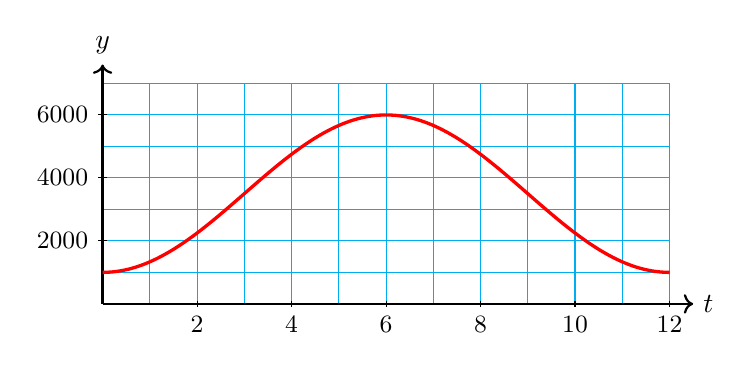
\begin{tikzpicture} [xscale=.6, yscale=.4]

\draw[cyan] (0,0) grid (12,7);
\draw[black,thick,->] (0,0) --(12.5,0) node[right]{$t$};
\draw[black,thick,->] (0,0) --(0,7.6) node[above]{$y$};

\foreach \x  in {2,4,...,12} {
 \draw[black] (\x,0.1)--+(0, -.2) node[below]{\small \x};
};
\foreach \y [evaluate=\y as \yi using int( 1000* \y )] in {2,4,6} {
 \draw[black] (0.1,\y)--+(-.2,0) node[left]{\small \yi};
};

\draw[samples=65,domain={0:12},smooth,variable=\x,red,very thick] plot ({\x},{3.5 - 2.5* cos( 30*\x)});

\end{tikzpicture}
\newline


hp4-3-61ans sinusoidal $y=51+21\sin 2\pi/12 t$

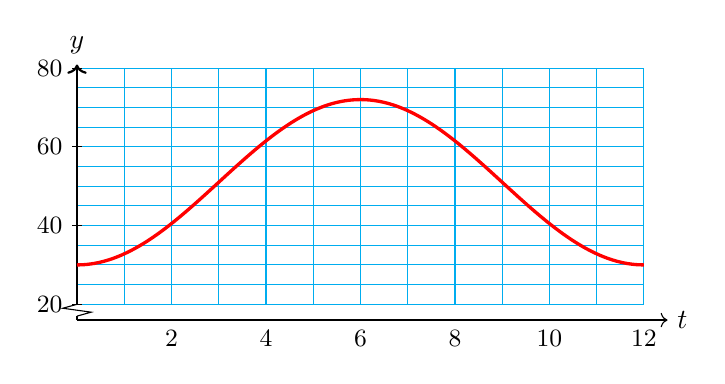
\begin{tikzpicture} [xscale=.6, yscale=.05]

\draw[cyan, ystep=5] (0,20) grid (12,80);
\draw[black,->] (0,16) --+(12.5,0) node[right]{$t$};
\draw[black,thick,->] (0,20) --(0,80.9) node[above]{$y$};
\draw[black] (0,20)--++(-.3, -1)--++(.6,-1)--++(-.3,-1);
\draw[black,thick] (0,16) --++(0,1);

\foreach \x  in {2,4,...,12} {
 \draw[black] (\x,16.1)--+(0, -.2) node[below]{\small \x};
};
\foreach \y in {20,40,...,80} {
 \draw[black] (0.1,\y)--+(-.2,0) node[left]{\small \y};
};

\draw[samples=65,domain={0:12},smooth,variable=\x,red,very thick] plot ({\x},{51 - 21* cos( 30*\x)});

\end{tikzpicture}
\newline


hp4-3-65 grid

\begin{tikzpicture} [xscale=.5, yscale=.4] 
\coordinate (O) at (0,0);
\draw[cyan] (0,0.9) grid (12,12);
\draw[black,->] (O) --+(12.5,0) node[right]{$m$};
\draw[black,thick,->] (O)++(0,.9) --++(0,12.) node[above]{$y$};
\draw[black] (O)++(0,.9)--++(-.3, -.2)--++(.6,-.2)--++(-.3,-.2) -- ++(0, -.3);

\foreach \x  in {2,4,...,12} {
 \draw[black] (\x,0)--+(0, -.2) node[below]{\footnotesize \x};
};
\foreach \y  [evaluate=\y as \yi using int(  \y /2 + 2)] in {2, 4, 6, ..., 12} {
 \draw[black] (0.1,\y)--+(-.2,0) node[left]{\footnotesize \yi};
};

% second grid
\coordinate (O) at (15,0);
\draw[cyan] (15,0.9) grid (27,12);
\draw[black,->] (O) --+(12.5,0) node[right]{$m$};
\draw[black,thick,->] (O)++(0,.9) --++(0,12.) node[above]{$y$};
\draw[black] (O)++(0,.9)--++(-.3, -.2)--++(.6,-.2)--++(-.3,-.2) -- ++(0, -.3);

\foreach \x  in {2,4,...,12} {
 \draw[black] (O)++(\x,0)--+(0, -.2) node[below]{\footnotesize \x};
};
\foreach \y  [evaluate=\y as \yi using int(  \y /2 + 14)] in {2, 4, 6, ..., 12} {
 \draw[black] (O)++(0.1,\y)--+(-.2,0) node[left]{\footnotesize \yi};
};

\end{tikzpicture}
\newline



hp4-3-65ans

\begin{tikzpicture} [xscale=.5, yscale=.4] 
\coordinate (O) at (0,0);
\draw[cyan] (0,0.9) grid (12,12);
\draw[black,->] (O) --+(12.5,0) node[right]{$m$};
\draw[black,thick,->] (O)++(0,.9) --++(0,12.) node[above]{$y$};
\draw[black] (O)++(0,.9)--++(-.3, -.2)--++(.6,-.2)--++(-.3,-.2) -- ++(0, -.3);

\foreach \x  in {2,4,...,12} {
 \draw[black] (\x,0)--+(0, -.2) node[below]{\footnotesize \x};
};
\foreach \y  [evaluate=\y as \yi using int(  \y /2 + 2)] in {2, 4, 6, ..., 12} {
 \draw[black] (0.1,\y)--+(-.2,0) node[left]{\footnotesize \yi};
};

% second grid
\coordinate (O) at (15,0);
\draw[cyan] (15,0.9) grid (27,12);
\draw[black,->] (O) --+(12.5,0) node[right]{$m$};
\draw[black,thick,->] (O)++(0,.9) --++(0,12.) node[above]{$y$};
\draw[black] (O)++(0,.9)--++(-.3, -.2)--++(.6,-.2)--++(-.3,-.2) -- ++(0, -.3);

\foreach \x  in {2,4,...,12} {
 \draw[black] (O)++(\x,0)--+(0, -.2) node[below]{\footnotesize \x};
};
\foreach \y  [evaluate=\y as \yi using int(  \y /2 + 14)] in {2, 4, 6, ..., 12} {
 \draw[black] (O)++(0.1,\y)--+(-.2,0) node[left]{\footnotesize \yi};
};

%\def\sunrise{{5.97, 6.43, 6.85, 6.98, 6.65, 6.1, 5.4, 4.9, 4.7, 4.72, 5.25, 5.62}}
\def\sunrise{{7.93, 8.87, 9.7, 9.97, 9.3, 8.13, 6.73, 5.73, 5.4, 5.43, 6.5, 7.23}}
%\def\sunset{{17.3, 16.8, 16.75, 17.1, 17.6, 18., 18.4, 18.8, 19.1, 19.1, 18.67, 18}}
\def\sunset{{6.67, 5.67, 5.5, 6.23, 7.23, 8., 8.83, 9.6, 10.23, 10.17, 9.33, 8}}

\foreach \x  in {0, 1,..., 11}
 \filldraw[red] (\x, \sunrise[\x]) ellipse (3.6pt and 4.5pt) ;

\draw[samples=65,domain={0:12},smooth,variable=\x,blue,very thick] plot ({\x},{7.57 + 2.3* sin( deg(.55*\x+.12)))});

\foreach \x [evaluate=\x as \y using (  \x  + 15)] in {0, 1,..., 11}
 \filldraw[red] (\y, \sunset[\x])  ellipse (3.6pt and 4.5pt) ;

\draw[samples=65,domain={0:12},smooth,variable=\x,blue,very thick] plot ({\x+15},{7.92 + 2.24* sin( deg(.49*\x-2.45)))});

\end{tikzpicture}
\newline


hp4-3-66 grid

\begin{tikzpicture} [xscale=.5, yscale=.4] 
\coordinate (O) at (0,0);
\draw[cyan] (0,0.9) grid (12,12);
\draw[black,->] (O) --+(12.5,0) node[right]{$m$};
\draw[black,thick,->] (O)++(0,.9) --++(0,12.) node[above]{$y$};
\draw[black] (O)++(0,.9)--++(-.3, -.2)--++(.6,-.2)--++(-.3,-.2) -- ++(0, -.3);

\foreach \x  in {2,4,...,12} {
 \draw[black] (\x,0)--+(0, -.2) node[below]{\footnotesize \x};
};
\foreach \y  [evaluate=\y as \yi using int(  \y /2 + 9)] in {2, 4, 6, ..., 12} {
 \draw[black] (0.1,\y)--+(-.2,0) node[left]{\footnotesize \yi};
};



\end{tikzpicture}
\newline



\end{document}
